\documentclass{../../zirkelblatt1718}
\graphicspath{{../}}
\usepackage{multicol}
\usepackage{tikz}
\usetikzlibrary{arrows,decorations.pathreplacing}
\usepackage{subfig}

\theoremstyle{definition}
\newtheorem{defn}{Definition}
\newtheorem{bsp}[defn]{Beispiel}

\theoremstyle{plain}
\newtheorem{prop}[defn]{Proposition}
\newtheorem{satz}[defn]{Satz}

\theoremstyle{remark}
\newtheorem{bem}[defn]{Bemerkung}
\newtheorem{aufg}[defn]{Aufgabe}
\newtheorem{tipp}[defn]{Tipp}
\newtheorem{motto}[defn]{Motto}

\renewcommand{\NN}{\mathbb{N}}
\newcommand{\RR}{\mathbb{R}}
\newcommand{\Slope}{S}
\newcommand{\Front}{F}
\newcommand{\Intersect}{\Delta}


\begin{document}

\maketitleCustom{Klassen 11/12}{\textbf{\textsf{%
  Der eulersche Pentagonalsatz \\
  \normalsize Korrespondenzzirkel vom 8. Dezember 2017}}}


\section{Problem}

Mir fehlt hier noch ein guter Aufhänger...

\begin{defn}
Eine Partition einer natürlichen Zahl $n$ ist ein Tupel $(n_1, n_2, \dots,
n_k)$ von natürlichen Zahlen mit $n_1  \geq n_2 \geq \dots \geq n_k > 0$
sodass $n_1 + n_2 + \dots + n_k = n$. Jedes $n_i$ in einer solchen Partition
heißt Teil der Partition. Man sagt, dass $(n_1, n_2, \dots, n_k)$ eine
Partition von $n$ in $k$ Teile ist.

Mit $p(n)$ bezeichnen wir die Anzahl der verschiedenen Partitionen einer
natürlichen Zahl $n$. Die Funktion $p \colon \NN \to \NN, n \mapsto p(n)$,
heißt die Partitionsfunktion.
\end{defn}

\begin{motto}
Eine Partition von $n$ ist eine Möglichkeit die Zahl $n$ als Summe von
positiven natürlichen Zahlen $n_1, n_2, \dots, n_k$ zu schreiben, wobei
Summen, die sich nur in ihrer Reihenfolge der Summanden unterscheiden, als
gleich angesehen werden.
\end{motto}

\begin{bsp}
 Als Beispiel listen wir mal alle $11$ Partitionen von $6$ auf:
 \begin{multicols}{3}
  \begin{itemize}
   \item[] $(6)$
   \item[] $(5,1)$
   \item[] $(4,2)$
   \item[] $(4,1,1)$
   \item[] $(3,3)$
   \item[] $(3,2,1)$
   \item[] $(3,1,1,1)$
   \item[] $(2,2,2)$
   \item[] $(2,2,1,1)$
   \item[] $(2,1,1,1,1)$
   \item[] $(1,1,1,1,1,1)$.
   \item[]
  \end{itemize}
 \end{multicols}
\end{bsp}

Einzelne Partitionen sind für uns eher uninteressant. Wir interessieren uns
dafür umso mehr um die Anzahl $p(n)$ von Partitionen einer beliebigen
natürlichen Zahl $n$. Wie Du Dir vorstellen kannst, wächst diese Anzahl
sehr schnell an. Hier ein paar Beispielswerte: $p(10) = 42$, $p(20) = 627$,
$p(30) = 5604$, $p(40) = 37 \, 338$ und $p(100) = 190 \, 569 \, 292$. Die
Anzahl der Partitionen der Zahl $10\,000$ hat bereits $107$ Stellen und die
Anzahl der Partitionen der Zahl $1\,000\,000$ hat $1108$ Stellen. Zum
Vergleich: Es wird vermutet, dass die Anzahl der Atome im Universum etwa $80$
bis $100$ Stellen hat. Lächerlich wenig sozusagen...

An sich ist es nicht schwer, $p(n)$ durch Auflisten aller Partitionen von $n$
herauszufinden, aber aufgrund der gewaltigen Anzahl an Möglichkeiten ist
dieser Ansatz praktisch nicht durchführbar. Gibt es andere Möglichkeiten?
Die Antwort ist glücklicherweise ja! Die drei genialen Mathematiker Hardy,
Ramanujan und Rademacher fanden folgende Formel:
$$
 p(n) = \cfrac{1}{\pi \sqrt{2}} \, \sum_{k=1}^\infty A_k(n) \ \sqrt{k} \ \cfrac{d}{dn} \! \! \left( \cfrac{\sinh \! \left(\cfrac{\pi}{k} \ \sqrt{\frac{2}{3} \left(n - \frac{1}{24} \right)}\right)}{\sqrt{n - \frac{1}{24}}} \right),
$$
wobei
$$
 A_k(n) = \sum_{h=1}^{k} \delta_{gcd(h,k), 1} \ \exp \! \left( \pi i \sum_{j=1}^{k-1} \frac{j}{k} \left(\frac{hj}{k} - \left\lfloor \frac{hj}{k} \right\rfloor -\frac{1}{2} \right) - \frac{2 \pi i h n}{k} \right).
$$
Wow! Bei dieser Formel können wir nur gemeinsam Staunen, denn leider
verstehen auch wir Zirkelleiter diese Formel nicht. Alleine darüber, wie man
mithilfe dieser Formel geschickt einen Wert berechnet, haben Mathematiker ganze
Arbeiten geschrieben.

Es gibt aber noch einen anderen Weg, den wir auch nachvollziehen können: Wir
können Rekursionen herleiten, mit deren Hilfe wir aus uns bereits bekannten
Werten der Partitionsfunktion neue Werte mit relativ wenig Aufwand berechnen
können. Bevor es die Formel von Hardy, Ramanujan und Rademacher gab, war
diese Möglichkeit die einzige praktikable, größere Werte der
Partitionsfunktion zu berechnen. Der Nachteil dieser Methode ist, wie wir sehen
werden, dass man alle (zumindest viele) kleineren Werte der Partitionsfunktion
kennen muss, bevor man den nächsten berechnen kann. Das soll uns aber nicht
stören.

\section{Herleitung von Rekursionsformeln}

Was jetzt kommt, hat auf den ersten Blick rein gar nichts mit unserer
Fragestellung zu tun: Wir multiplizieren mal
\footnotesize
$$
 P(X) := (1 + X + X^2 + \dots + X^i + \dots)(1 + X^2 + X^4 + \dots + X^{2j} + \dots)(1 + X^3 + X^6 + \dots + X^{3k} + \dots) \cdots
$$
\normalsize
aus. Vorsicht:
Dieses Produkt hat unendlich viele Faktoren und jeder Faktor wiederum endlich
viele Summanden. Das ist vielleicht ungewöhnlich, aber wir können ganz
normal damit rechnen. Wir können natürlich nie komplett ausmultiplizieren,
aber wir können durchaus die ersten Koeffizienten berechnen:
\begin{align*}
 P(X) =  1 + X + 2X^2 + 3X^3 + 5X^4 + \dots
\end{align*}
Schauen wir uns mal ganz genau an, wie wir oben den Koeffizienten vor $X^4$
berechnen: Zu diesem erhalten wir wie Du weißt einen Beitrag, wenn wir aus
dem ersten Faktor $X^4$ und aus allen anderen $1$ auswählen, oder wenn wir
aus dem ersten Faktor $X$, aus dem dritten $X^3$ und aus allen anderen $1$
auswählen und so weiter. Zur besseren Übersicht hier eine Tabelle mit allen
Möglichkeiten:

$\begin{array}{c|c|c|c|c}
 \text{$1$. Faktor} & \text{$2$. Faktor} & \text{$3$. Faktor} & \text{$4$. Faktor} & \text{alle anderen Faktoren}\\
 \hline
 X^4 & 1 & 1 & 1 & 1 \\
 X^2 & X^2 & 1 & 1 & 1 \\
 X & 1 & X^3 & 1 & 1 \\
 1 & X^4 & 1 & 1 & 1 \\
 1 & 1 & 1 & X^4 & 1
\end{array}$\\[\baselineskip]

Wie Du siehst, steht in der letzten Spalte immer nur eine $1$, da die
Exponenten aller anderen $X$-Potenzen in diesen Faktoren schon zu groß
sind.\footnote{ Das ist übrigens der Grund, warum wir so gut mit diesem
Produkt umgehen können. Zwar ist das Produkt \glqq unendlich lang\grqq\ \!,
aber für jeden einzelnen Koeffizienten in der ausmultiplizierten Form
brauchen wir nur endlich viele Faktoren zu beachten.} Wir können uns also auf
die ersten $4$ Faktoren konzentrieren. Wenn wir nur die ersten vier Faktoren
ausmultiplizieren, so haben die Exponenten $k$ in der ausmultiplizierten Form
folgende Gestalt:
$$
 k = 1 k_1 + 2 k_2 + 3 k_3 + 4 k_4
$$
Dabei ist $k_i$ der Exponent der $X$-Potenz, welche wir im $i$-ten Faktor
gewählt haben.\footnote{ Die $1$ sehen wir dabei als $X^0$ an.}
Wir suchen speziell nach solchen Kombinationen, sodass der Exponent gleich $4$
ist, wir erhalten also die Gleichung
$$
 4 = 1 k_1 + 2 k_2 + 3 k_3 + 4 k_4.
$$
Wir müssen also passende Werte für die $k_i$ finden. Jetzt kommt der Clou:
Jede solche Lösung entspricht einer Partition der Zahl $4$. Wir können
nämlich $k_i$ auch als Anzahl der Teile der Größe $i$ sehen. Da die
$k_i$ eine Lösung der Gleichung sind, summieren sich die Teile dann genau zu
$4$. Zeit für ein konkretes Beispiel: Aus
$$
 4 = 1 \cdot 1 + 2 \cdot 0 + 3 \cdot 1 + 4 \cdot 0
$$
erhalten wir die Partition der $4$ mit einem Teil der Größe $1$ und mit
einem Teil der Größe $3$, also $4 = 3 + 1$ bzw. $(3,1)$ in der ganz
korrekten Tupelschreibweise. In der Tabelle ist eine Übersicht über alle
Partitionen der $4$.

$\begin{array}{c|c|c|c|c|r}
 \text{$1$. Faktor} & \text{$2$. Faktor} & \text{$3$. Faktor} & \text{$4$. Faktor} & (k_1,k_2,k_3,k_4) & \text{Partition}\\
 \hline
 X^4 & 1 & 1 & 1 & (4,0,0,0) & 1+1+1+1\\
 X^2 & X^2 & 1 & 1 & (2,1,0,0) & 2+1+1\\
 X & 1 & X^3 & 1 & (1,0,1,0) & 3+1\\
 1 & X^4 & 1 & 1 & (0,2,0,0) & 2+2\\
 1 & 1 & 1 & X^4 & (0,0,0,1) & 4
\end{array}$\\[\baselineskip]

% Nur zur Hälfte ausfüllen und den Rest als Aufgabe?

Wir erhalten natürlich auch für andere Zahlen als die $4$ Partitionen. Wenn
wir Partitionen für $n$ auf diese Art und Weise finden wollen, können wir
uns auf die ersten $n$ Faktoren von $P(X)$ beschränken und erhalten
Gleichungen der Form
$$
 n = 1 k_1 + 2 k_2 + 3 k_3 + \dots + n k_n.
$$

Das Tolle dabei: Wir lassen keine Partition aus, erhalten auf diese Weise also
wirklich jede Partition! Gleichzeitig erhalten wir jede Partition nur genau
einmal. Was bedeutet das für den Koeffizienten vor $X^n$ in $P(X)$? Dieser
ist nichts anderes als $p(n)$, die Anzahl der Partitionen von $n$, d.\,h.
$$
 P(X) = p(0) + p(1)X + p(2)X^2 + p(3)X^3 + \dots
$$
Wenn wir also wissen wollen, wie viele Partitionen die Zahl $10$ hat, können
wir einfach beginnen, die ersten $10$ Faktoren von $P(X)$ auszumultiplizieren
und uns anschließend ansehen, welcher Koeffizient vor $X^{10}$ steht, das
ist die Antwort. Das ist aber noch nicht zufriedenstellend, denn kein Mensch
hat Lust ein solch unübersichtliches Produkt zu berechnen.\\ Man nennt $P(X)$
auch die erzeugende Funktion der Partitionsfunktion. Das ist aber nicht so zu
verstehen, dass wir in diese erzeugende Funktion $P(X)$ irgendwelche Werte
für $X$ einsetzen möchten, das ergibt in den meisten Fällen überhaupt
keinen Sinn. Man kann sich eine solche erzeugende Funktion eher als
Wäscheleine vorstellen, an der man die Folgenglieder einer Folge der Reihe
nach neben den Potenzen einer Variable aufhängt, so wie wir es (unbewusst)
auch getan haben. Die Potenzen dieser Variable haben keine Bedeutung, sie
helfen uns nur, den Überblick zu behalten und sorgen für Ordnung auf der
Leine. Das verblüffende ist, dass man mit erzeugenden Funtionen sinnvolle
Ergebnisse über die Folge herausfinden kann, indem man einfach mit ihr
rechnet, als wäre sie eine gewöhnliche Funktion. Dabei hat man oft kein ein
Gefühl dafür, was diese Rechenoperationen auf der Folge direkt für
Auswirkungen haben. Genau das werden wir jetzt auch machen.

Betrachten wir den $m$-ten Faktor von $P(X)$. Die Multiplikation von diesem mit
$(1-X^m)$ liefert:
\begin{align*}
 &(1 + X^m + X^{2m} + X^{3m} + X^{4m} + \dots ) (1 - X^m) \\
 = &(1 + X^m + X^{2m} + X^{3m} + X^{4m} + \dots ) - (X^m + X^{2m} + X^{3m} + X^{4m} + X^{5m} \dots )
 = 1.
\end{align*}
Das ermöglicht es uns, diesen Faktor sehr kompakt zu schreiben, indem wir
einfach durch $(1-X^m)$ teilen:
$$
 (1 + X^m + X^{2m} + X^{3m} + X^{4m} + \dots ) = \cfrac{1}{1 - X^m}.
$$
Wenn wir das für jeden Faktor von $P(X)$ machen, können wir
$$
 P(X) = \cfrac{1}{(1-X)(1-X^2)(1-X^3) \cdots}
$$
schreiben. Das scheint uns erst mal nichts zu bringen. Doch Leonhard Euler
entdeckte einen Zusammenhang zwischen dem Nenner $(1-X)(1-X^2)(1-X^3) \cdots$
von $P(X)$ und den sogenannten Pentagonalzahlen, die Du vielleicht schon mal
kennen gelernt hast. Durch Ausnutzung dieses Zusammenhangs können wir uns
dann endlich Rekursionsformeln herleiten. Zunächst sollten wir aber klären,
was Pentagonalzahlen überhaupt sind.

\begin{defn}\textbf{Pentagonalzahlen}\\
 Als Pentagonalzahlen bezeichnen wir natürliche Zahlen  der Form
 $$
  n = \frac{k(3k \pm 1)}{2}
 $$
 für ein $k$, wobei $\pm$ entweder für $+$ oder für $-$ steht.\footnote{
 Es handelt sich tatsächlich immer um eine natürliche Zahl und nicht um
 einen Bruch.: Wenn $k$ gerade ist, ist das klar. Ansonsten ist aber $3k \pm 1$
 gerade, und somit ist $n$ auch in diesem Fall eine natürliche Zahl.} Oft
 werden die Zahlen der Form $\frac{k(3k - 1)}{2}$ als \glqq echte \grqq\
 Pentagonalzahlen bezeichnet, während die Zahlen der Form $\frac{k(3k +
 1)}{2}$ als erweiterte Pentagonalzahlen bezeichnet werden. Die Folge der
 echten Pentagonalzahlen beginnt mit $0,\,1,\,5,\,12,\,22,\dots$, die der
 erweiterten Pentagonalzahlen mit $0,\,2,\,7,\,15,\,26,\dots$. Das folgende
 Bild erklärt die Herkunft des Namens für die echten Pentagonalzahlen.
 \begin{center}
  % http://www.icoachmath.com/math_dictionary/pentagonal_number.html
  % Erwähnen?
  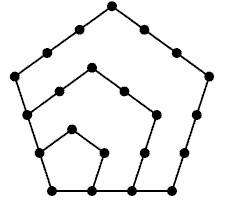
\includegraphics[width=4.5cm,scale=0.8]{Pentagonal_Numbers.jpg}
 \end{center}
 Zähle doch mal, aus  wie vielen Punkten die einzelnen regelmäßigen
 Fünfecke (= Pentagon) bestehen. Richtig, aus $1,\,5,\,12,\,22,\dots$
 Punkten.
\end{defn}

\begin{satz}\textnormal{\textbf{Eulerscher Pentagonalsatz}}\\
Es gilt
$$
 (1-X)(1-X^2)(1-X^3) \cdots = 1 + \sum_{k=1}^{\infty} (-1)^k \Big(X^{k(3k+1)/2} + X^{k(3k-1)/2}\Big).
$$
Beachte: Die Exponenten auf der rechten Seite sind gerade die Pentagonalzahlen.
\end{satz}

\begin{proof}
 Der erste Schritt zum Durchblick ist es, eine geeignete Interpretation für
 die linke Seite der Gleichung zu finden. Wir wollen schließlich irgendwie
 wieder zu unseren Partitionen kommen. Wir können uns nochmal das Produkt
 $$
  (1 + X + X^2 + \dots + X^i + \dots)(1 + X^2 + X^4 + \dots + X^{2j} + \dots)(1 + X^3 + X^6 + \dots + X^{3k} + \dots) \cdots
 $$
 betrachten, wo wir bereits einen solchen Zusammenhang herstellen konnten. Die
 Wahl des $i$-ten Summanden im $j$-ten Faktor entsprach in der zugehörigen
 Partition der Wahl von $i-1$ Teilen der Größe $j$. Im Produkt (wir
 ignorieren erstmal die Minuszeichen)
 $$
  (1+X)(1+X^2)(1+X^3) \cdots
 $$
 haben wir pro Faktor immer nur zwei Summanden zur Auswahl. Für die dadurch
 beschriebenen Partitionen heißt das, dass wir zu jeder Größe
 entweder kein Teil oder genau ein Teil aufnehmen können, nicht aber mehrere.
 Das bedeutet, dass wir so nur Partitionen beschreiben, die aus lauter
 verschieden großen Teilen bestehen. Als erzeugende Funktion geschrieben:
 $$
  (1+X)(1+X^2)(1+X^3) \cdots = p_{dist}(0) + p_{dist}(1)X + p_{dist}(2)X^2 + p_{dist}(3)X^3 + \dots,
 $$
 wobei $p_{dist}(n)$ die Anzahl der Partitionen von $n$ in verschieden
 große Teile ist.\footnote{ Zum Beispiel hat die Zahl $4$ genau zwei solche
 Partitionen, nämlich $(3,1)$ und $(4)$. Bei allen anderen Partitionen
 $(1,1,1,1)$, $(2,1,1)$ und $(2,2)$ der $4$ dagegen treten einige Teile
 gleicher Größe mehrfach auf.} Wenn wir das verstanden haben, können
 wir auch über die Minuszeichen in
 $$
  (1-X)(1-X^2)(1-X^3) \cdots
 $$
 nachdenken: Das Vorzeichen eines Koeffizienten in der ausmultiplizierten Form
 ist abhängig von der Anzahl der Teile der beschriebenen Partition. So
 erhalten die Terme, die zu Partitionen mit gerade vielen Teilen
 korrespondieren, positives Vorzeichen, während die Terme, die Partitionen
 mit ungerader Teileanzahl beschreiben, negatives Vorzeichen erhalten.
 Überlege Dir das an ein paar Beispielen. Wir erhalten
 $$
  (1-X)(1-X^2)(1-X^3) \cdots = p_{dist}^{g-u}(0) + p_{dist}^{g-u}(1)X + p_{dist}^{g-u}(2)X^2 + p_{dist}^{g-u}(3)X^3 + \cdots,
 $$
 wobei $p_{dist}^{g-u}(n)=p_{dist}^{g}(n) - p_{dist}^{u}(n)$ die Anzahl der
 Partitionen von $n$ in verschieden große Teile mit gerader Anzahl von
 Teilen minus die Anzahl der Partitionen von $n$ in verschieden große Teile
 mit ungerader Anzahl von Teilen ist.

 Wir werden sehen, dass $p_{dist}^{g-u}(n) \in \{-1, 0 ,1\}$ für alle $n$
 ist, und dass $p_{dist}^{g-u}(n) \neq 0$ nur gilt, wenn $n$ eine
 Pentagonalzahl ist. Dazu benötigen wir Ferrers Diagramme, die Partitionen
 visualisieren.

 \begin{defn}\textbf{Ferrers Diagramme}\\
  Ein Ferrer Diagramm zu einer Partition $(n_1, n_2, \dots, n_k)$ von $n$ ist
  ein Säulendiagramm mit $k$ Säulen, wobei die $i$-te Säule $n_i$
  Kästchen hoch ist. Wir veranschaulichen dies mal anhand der Partitionen
  $(8,7,6,6,5,3)$ und $(8,7,6,5,4,3)$ der Zahlen $35$ und $30$:

  \begin{figure}[h]
  \centering
  \scalebox{0.5}{
   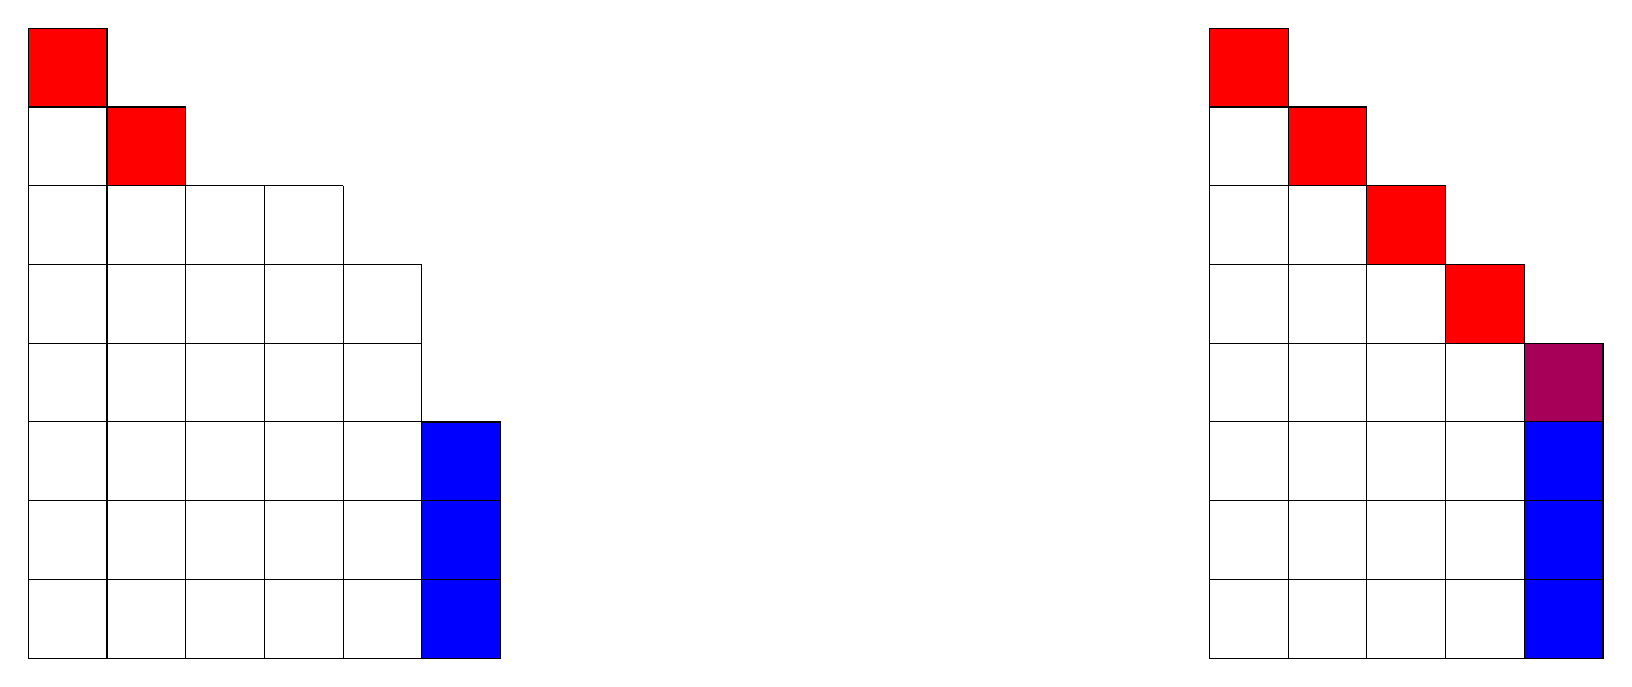
\begin{tikzpicture}
    %% Markierung
    \draw[fill=red] (0,7) rectangle (1,8);
    \draw[fill=red] (1,6) rectangle (2,7);
    \draw[fill=blue] (5,0) rectangle (6,3);

   % Achsenbeschriftungen
    %\foreach \x in {0,1,2,3,4,5} \foreach \y in {9,8,7,4,3,1} \fill[color=black] (\x,\y) -- (0pt,0pt)
    \draw[color=black] (0,0) grid (1,8);
    \draw[color=black] (1,0) grid (2,7);
    \draw[color=black] (2,0) grid (3,6);
    \draw[color=black] (3,0) grid (4,6);
    \draw[color=black] (4,0) grid (5,5);
    \draw[color=black] (5,0) grid (6,3);

    %% Markierung
    \draw[fill=red] (15,7) rectangle (16,8);
    \draw[fill=red] (16,6) rectangle (17,7);
    \draw[fill=red] (17,5) rectangle (18,6);
    \draw[fill=red] (18,4) rectangle (19,5);
    \draw[fill=red!65!blue] (19,3) rectangle (20,4);
    \draw[fill=blue] (19,0) rectangle (20,3);

    %% Diagramm
    \draw[color=black] (15,0) grid (16,8);
    \draw[color=black] (16,0) grid (17,7);
    \draw[color=black] (17,0) grid (18,6);
    \draw[color=black] (18,0) grid (19,5);
    \draw[color=black] (19,0) grid (20,4);
   \end{tikzpicture}}
  \end{figure}

  Die Kästchen der $k$-ten (letzten) Säule nennen wir Front (im Bild blau
  markiert). Die jeweils obersten Kästchen der ersten Säulen, sodass die
  jeweils folgende Säule genau ein Kästchen niedriger ist, werden ebenfalls
  zusammengefasst. Diese werden wir als Schräge bezeichnen. Im Bild sind
  diese Kästchen rot markiert. Es kann sein, dass sich die Front und die
  Schräge ein Kästchen teilen, wie das lila farbene Kästchen bei der
  rechts abgebildeten Partition.\\
  Die Anzahl der Kästchen der Front, der Schräge bzw. des Schnitts werden
  wir mit $\Front$, $\Slope$ bzw. $\Intersect$ abkürzen.
 \end{defn}


 Wir halten zunächst einige kleine Beobachtungen fest: Eine Partition von $n$
 ist genau dann eine Partition in verschieden große Teile, wenn alle
 Säulen im zugehörigen Ferrers Diagramm unterschiedlich hoch sind. Ferner
 ist die Anzahl der Kästchen des Ferrers Diagramm gleich $n$. Außerdem
 ist $\Intersect = 0$ oder $\Intersect = 1$, d.\,h. die Front und Schräge
 können sich maximal ein Kästchen teilen. Die Anzahl der Kästchen der
 Schräge ist kleiner gleich der Anzahl der Säulen $k$, d.\,h. $\Slope \leq
 k$ und Gleichheit tritt genau dann auf, wenn $\Intersect = 1$.

 Wie können uns diese Diagramme nun weiterhelfen? Zur Erinnerung: Wir wollten
 herausfinden, was $p_{dist}^{g-u}(n) = p_{dist}^{g}(n) - p_{dist}^{u}(n)$ ist.
 Wir werden uns also nur Ferrers Diagramme mit unterschiedlich hohen Säulen
 ansehen. Wir könnten nun versuchen $p_{dist}^{g}(n)$ und $p_{dist}^{u}(n)$
 seperat zu berechnen und danach die Differenz bilden. Wir werden anders
 verfahren.

 Unser Trick wird sein, soweit möglich zu versuchen, jeder Partition $p$ von
 $n$ in verschieden große Teile eine \glqq Partner\grqq\ \!-Partition $p^*$
 von $n$ zuzuordnen, die ebenfalls nur aus verschieden großen Teilen
 besteht. Dabei soll genau eine der verpartnerten Partitionen $p$ und $p^*$
 ungerade viele Teile besitzen und die andere entsprechend gerade viele Teile
 haben. Außerdem soll der Partner von $p^*$ wieder $p$ sein (verpartnerte
 Partitionen sind sich treu), d.\,h. $\left(p^*\right)^* = p$. Wie im echten
 Leben werden einige Partitionen keinen Partner finden, aber die meisten
 Partitionen werden nicht alleine bleiben.

 Was wird uns das bringen? Wir müssen zu einer Zahl $n$ nur wissen, wie viele
 Partitionen von $n$ partnerlos bleiben. Denn von einem Partitionen-Paar
 $(p,p^*)$ trägt genau eine Partition zu $p_{dist}^{g}(n)$ und die andere zu
 $p_{dist}^{u}(n)$ bei. Zusammen genommen wird das Paar also keinen Beitrag zur
 Differenz $p_{dist}^{g-u}(n) = p_{dist}^{g}(n) - p_{dist}^{u}(n)$ leisten.

 Wir werden die gesuchte Zuordnung nun am Beispiel der Partition $p =
 (11,10,9,8,6,5,3)$ von $52$ motivieren. Wie wir anhand des zugehörigen
 Ferrers Diagramm leicht ablesen können, ist die Front hier kleiner als die
 Schräge:

 \begin{figure}[h]
  \centering
  \scalebox{0.5}{
  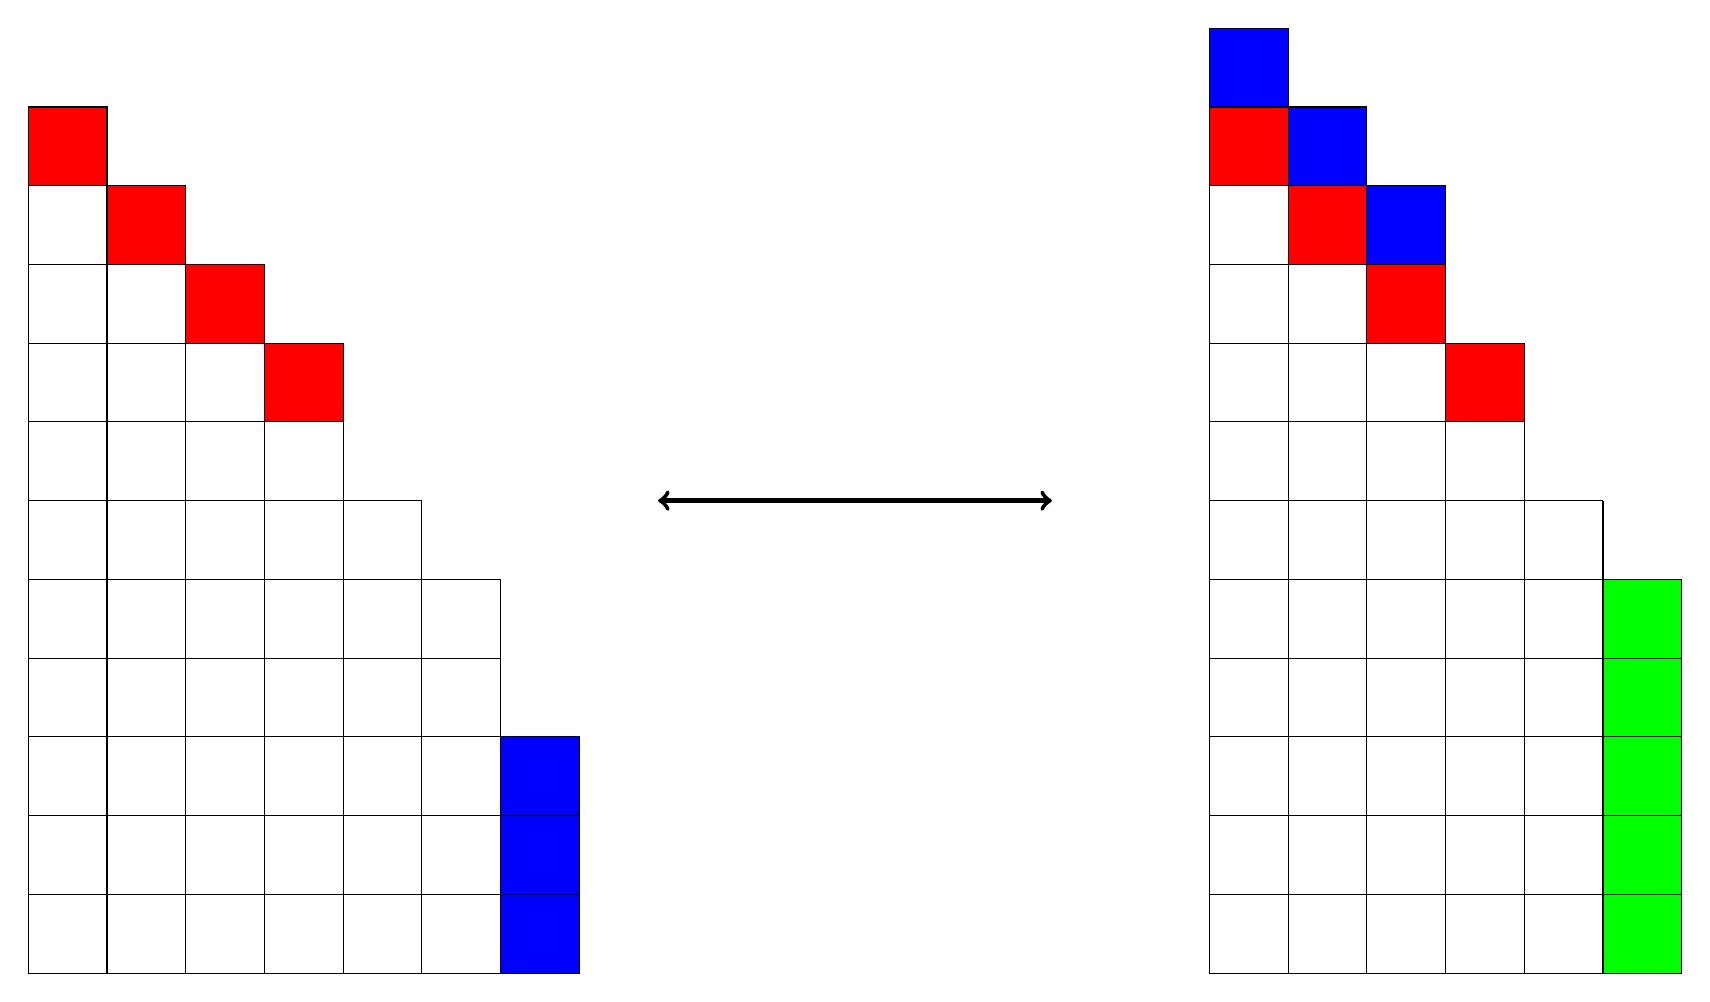
\begin{tikzpicture}
   %% Markierung
   \draw[fill=red] (0,10) rectangle (1,11);
   \draw[fill=red] (1,9) rectangle (2,10);
   \draw[fill=red] (2,8) rectangle (3,9);
   \draw[fill=red] (3,7) rectangle (4,8);
   \draw[fill=blue] (6,0) rectangle (7,3);

   %% Diagramm
   \draw[color=black] (0,0) grid (1,11);
   \draw[color=black] (1,0) grid (2,10);
   \draw[color=black] (2,0) grid (3,9);
   \draw[color=black] (3,0) grid (4,8);
   \draw[color=black] (4,0) grid (5,6);
   \draw[color=black] (5,0) grid (6,5);
   \draw[color=black] (6,0) grid (7,3);


   %% Markierung
   \draw[fill=red] (15,10) rectangle (16,11);
   \draw[fill=red] (16,9) rectangle (17,10);
   \draw[fill=red] (17,8) rectangle (18,9);
   \draw[fill=red] (18,7) rectangle (19,8);
   \draw[fill=blue] (15,11) rectangle (16,12);
   \draw[fill=blue] (16,10) rectangle (17,11);
   \draw[fill=blue] (17,9) rectangle (18,10);
   \draw[fill=green] (20,0) rectangle (21,5);

   %% Diagramm
   \draw[color=black] (15,0) grid (16,12);
   \draw[color=black] (16,0) grid (17,11);
   \draw[color=black] (17,0) grid (18,10);
   \draw[color=black] (18,0) grid (19,8);
   \draw[color=black] (19,0) grid (20,6);
   \draw[color=black] (20,0) grid (21,5);

   \draw[ultra thick,<->] (8,6) -- (13,6);
  \end{tikzpicture}}
 \end{figure}

 \newpage

 Sehen wir uns nun an, was passiert, wenn wir die Front auf Schräge legen,
 wie in der Abbildung eingezeichnet. Die so erhaltene Partition
 $(12,11,10,8,6,5)$ ist wieder eine Partition von $52$, denn die Anzahl der
 Kästchen haben wir ja nicht verändert. Diese hat genau eine Säule bzw.
 Teil weniger (aus einer geraden/ungeraden Teileanzahl wird eine
 ungerade/gerade Teileanzahl). Ferner sind noch immer alle Säulen bzw. Teile
 verschieden groß. Somit ist die Partition $(12,11,10,8,6,5)$ ein
 geeigneter Partner für die Partition $(11,10,9,8,6,5,3)$.

 Wie sähe nun der Partner von $(11,10,9,8,6,5,3)$ aus? Dieser sollte ja
 wieder $p$ sein. Wir können nicht einfach erneut die Front von
 $(11,10,9,8,6,5,3)$ (grün im Bild) wieder auf ihre Schräge legen, denn die
 Front von $(11,10,9,8,6,5,3)$ ist größer als ihre Schräge.
 Andererseits hätten wir das gar nicht gewollt, denn wir wollen ja wieder zu
 $p$ zurück. Ist die Front also zu groß um sie auf die Schräge zu
 legen, so können wir es umgekehrt probieren, und die Schräge vor die Front
 stellen. Wir erhalten folgende Idee für eine Zuordnung von Partnern:

 Der Partner $p^*$ einer Partition $p$ (falls existent) ist gegeben durch
 $$p^* = \footnotesize
 \begin{cases}
  \text{die Partition, die aus } p \text{ durch Legen der Front auf die Schräge hervorgeht, falls möglich;}\\
  \text{sonst die Partition, die aus } p \text{ durch Stellen der Schräge vor die Front hervorgeht, falls möglich.}
  %p \text{ selbst in allen sonstigen Fällen. (In diesem Fall hat $p$ keinen echten Partner.)}
 \end{cases}
 $$

 Wir werden nun zeigen, dass diese Idee tatsächlich zum Erfolg führt. Wir
 werden eine Fallunterscheidung durchführen und die Partitionen von $n$ in
 verschieden große Teile in drei Typen einteilen.

 \begin{itemize}
  \item[Typ I:] $\Slope \geq \Front + \Intersect$\\[0.5\baselineskip]
   Behauptung: Das sind genau die Partitionen, für welche es möglich ist,
   die Front auf die Schräge zu legen.

   Wir werden die beiden Fälle $\Intersect = 0$ und $\Intersect = 1$
   gesondert betrachten, um den Überblick zu wahren und uns zunächst zwei
   Beispiele ansehen.

  \begin{figure}[h]
  \centering
  \scalebox{0.5}{
  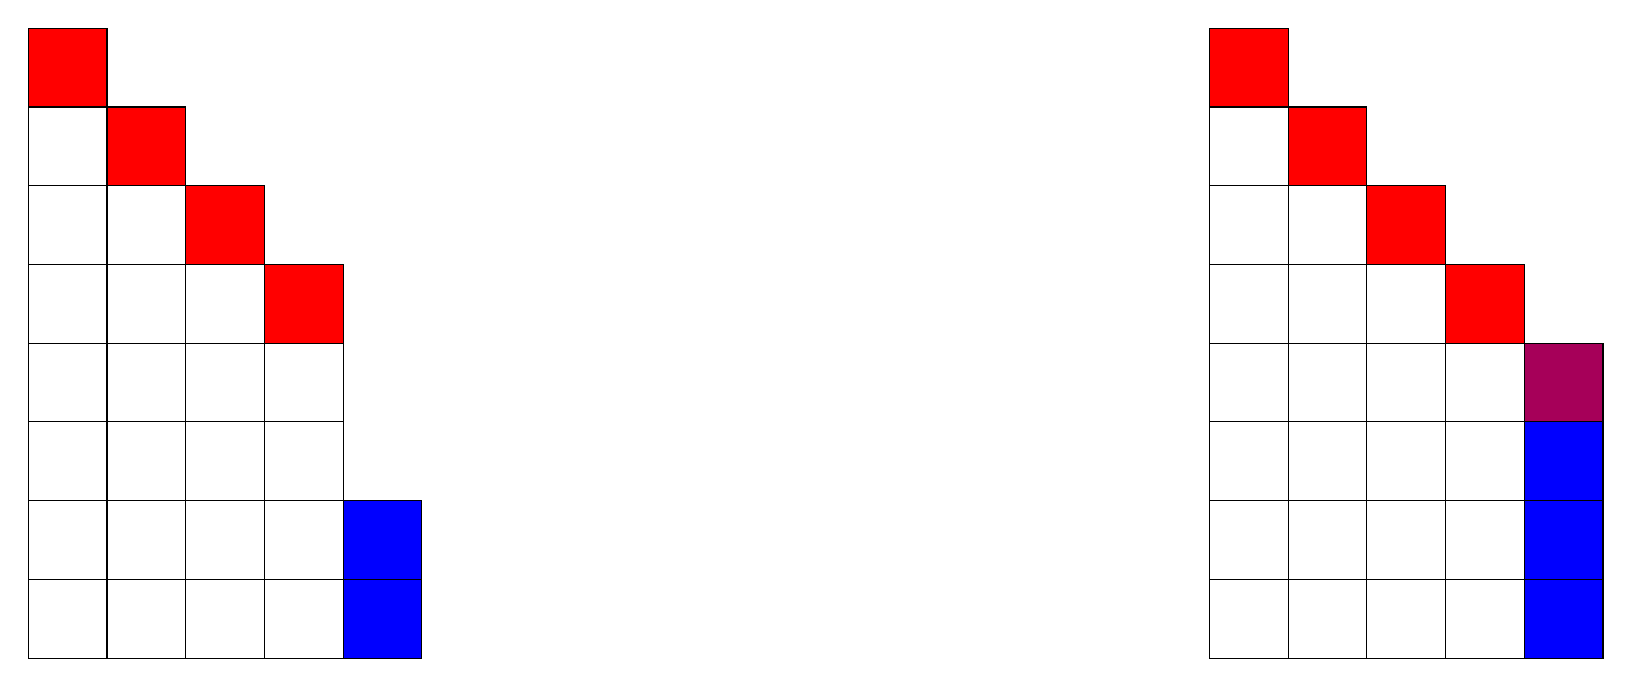
\begin{tikzpicture}
   %% Markierung
   \draw[fill=red] (0,7) rectangle (1,8);
   \draw[fill=red] (1,6) rectangle (2,7);
   \draw[fill=red] (2,5) rectangle (3,6);
   \draw[fill=red] (3,4) rectangle (4,5);
   \draw[fill=blue] (4,0) rectangle (5,2);

   %% Diagramm
   \draw[color=black] (0,0) grid (1,8);
   \draw[color=black] (1,0) grid (2,7);
   \draw[color=black] (2,0) grid (3,6);
   \draw[color=black] (3,0) grid (4,5);
   \draw[color=black] (4,0) grid (5,2);


   %% Markierung
   \draw[fill=red] (15,7) rectangle (16,8);
   \draw[fill=red] (16,6) rectangle (17,7);
   \draw[fill=red] (17,5) rectangle (18,6);
   \draw[fill=red] (18,4) rectangle (19,5);
   \draw[fill=blue] (19,0) rectangle (20,3);
   \draw[fill=red!65!blue] (19,3) rectangle (20,4);

   %% Diagramm
   \draw[color=black] (15,0) grid (16,8);
   \draw[color=black] (16,0) grid (17,7);
   \draw[color=black] (17,0) grid (18,6);
   \draw[color=black] (18,0) grid (19,5);
   \draw[color=black] (19,0) grid (20,4);
  \end{tikzpicture}}
 \end{figure}

  In beiden Beispielen können wir die gesammte Front auf Schräge legen,
  diese ist groß genug.
  %Wir können aber nicht Schräge vor die Front stellen, denn diese ist zu
  %klein (die Säulen müssen nach ihrer Höhe sortiert bleiben und echt
  %kleiner werden.)
  Wir erhalten für unsere Beispiele die folgenden Partitionen:

  \begin{figure}[h]
  \centering
  \scalebox{0.5}{
  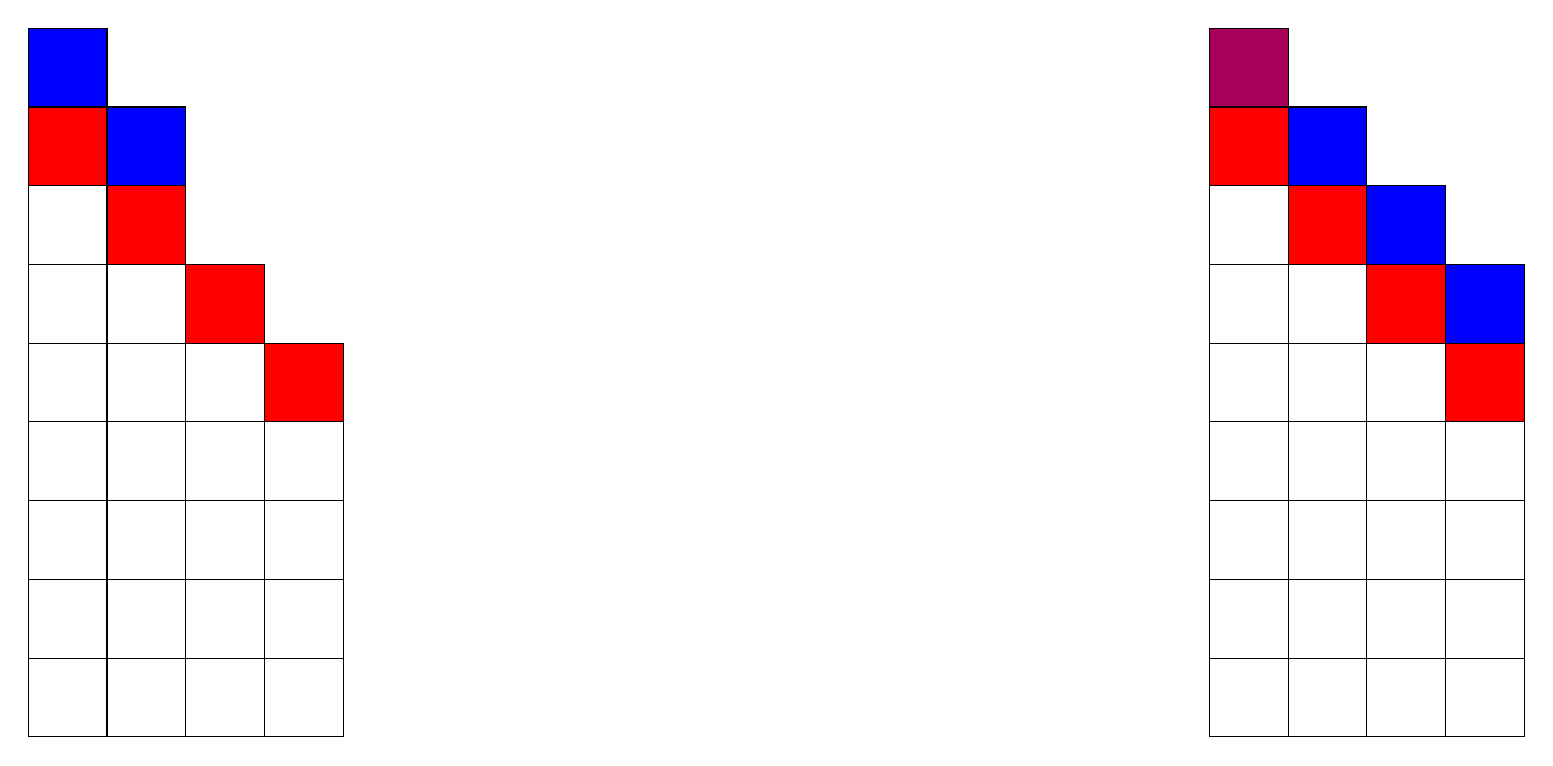
\begin{tikzpicture}
   %% Markierung
   \draw[fill=red] (0,7) rectangle (1,8);
   \draw[fill=red] (1,6) rectangle (2,7);
   \draw[fill=red] (2,5) rectangle (3,6);
   \draw[fill=red] (3,4) rectangle (4,5);
   \draw[fill=blue] (0,8) rectangle (1,9);
   \draw[fill=blue] (1,7) rectangle (2,8);

   %% Diagramm
   \draw[color=black] (0,0) grid (1,9);
   \draw[color=black] (1,0) grid (2,8);
   \draw[color=black] (2,0) grid (3,6);
   \draw[color=black] (3,0) grid (4,5);


   %% Markierung
   \draw[fill=red] (15,7) rectangle (16,8);
   \draw[fill=red] (16,6) rectangle (17,7);
   \draw[fill=red] (17,5) rectangle (18,6);
   \draw[fill=red] (18,4) rectangle (19,5);
   \draw[fill=red!65!blue] (15,8) rectangle (16,9);
   \draw[fill=blue] (16,7) rectangle (17,8);
   \draw[fill=blue] (17,6) rectangle (18,7);
   \draw[fill=blue] (18,5) rectangle (19,6);

   %% Diagramm
   \draw[color=black] (15,0) grid (16,9);
   \draw[color=black] (16,0) grid (17,8);
   \draw[color=black] (17,0) grid (18,7);
   \draw[color=black] (18,0) grid (19,6);
  \end{tikzpicture}}
 \end{figure}

%    Nicht möglich dagegen ist folgendes:
%
%    \begin{figure}[h]
%     \centering
%     \scalebox{0.5}{
%     \begin{tikzpicture}
%      %% Markierung
%      \draw[fill=blue] (4,0) rectangle (5,2);
%      \draw[fill=red] (5,0) rectangle (6,4);
%
%      %% Diagramm
%      \draw[color=black] (0,0) grid (1,7);
%      \draw[color=black] (1,0) grid (2,6);
%      \draw[color=black] (2,0) grid (3,5);
%      \draw[color=black] (3,0) grid (4,4);
%      \draw[color=black] (4,0) grid (5,2);
%      \draw[color=black] (5,0) grid (6,4);
%
%
%      %% Markierung
%      \draw[fill=blue] (19,0) rectangle (20,3);
%      \draw[fill=red!65!blue] (19,3) rectangle (20,4);
%      \draw[fill=red] (20,0) rectangle (21,4);
%
%      %% Diagramm
%      \draw[color=black] (15,0) grid (16,7);
%      \draw[color=black] (16,0) grid (17,6);
%      \draw[color=black] (17,0) grid (18,5);
%      \draw[color=black] (18,0) grid (19,4);
%      \draw[color=black] (19,0) grid (20,4);
%      \draw[color=black] (20,0) grid (21,4);
%
%
%      %% Durchstreichen
%      \draw[color=red!65!black] (-1.7,-1.7) -- (7.7,7.7);
%      \draw[color=red!65!black] (-1.7,7.7) -- (7.7,-1.7);
%
%      \draw[color=red!65!black] (13.7,-1.7) -- (22.7,7.7);
%      \draw[color=red!65!black] (13.7,7.7) -- (22.7,-1.7);
%     \end{tikzpicture}}
%    \end{figure}

  Etwas konkreter: Wir müssen sicherstellen, dass die Front aus weniger oder
  genauso vielen Kästchen besteht wie der Teil von Schräge, der nach
  Entfernen der Front übrig bleibt.

  Falls $\Intersect = 0$, sich die Front und die Schräge also kein Kästchen
  teilen, bleibt nach Entfernen der Front die gesamte Schräge übrig. In
  diesem Fall muss folglich $\Slope \geq \Front$ gelten. Ist dagegen
  $\Intersect = 1$, so bleiben von Schräge nach Entfernen der Front nur noch
  $\Slope - 1$ Kästchen übrig, also muss in diesem Fall $\Slope - 1 \geq
  \Front$ gelten. In beiden Fällen gilt also $\Slope - \Intersect \geq
  \Front$ bzw. $\Slope \geq \Front + \Intersect$. Damit ist obige Behauptung
  gezeigt.

  Wir wollen noch mehr: Sei $p=(n_1,n_2,\dots,n_k)$ unsere Partition von Typ I
  und $p^* = (n_1^*,n_2^*,\dots,n_{k-1}^*)$ ihr Partner, den wir durch Legen
  der Front auf die Schräge erhalten. Beachte dass $p^*$ genau eine Säule
  weniger als $p$ besitzt. Wir bezeichnen mit $\Slope^*$, $\Front^*$ bzw.
  $\Intersect^*$ die Schräge, die Front bzw. den Schnitt von $p^*$. Damit
  gilt
  \begin{equation}\label{eq_Legen}
   \Slope^* = \Front \qquad \text{und} \qquad \Front^* > \Front.
  \end{equation}
  Wir werden nun folgende Behauptung zeigen: Es gilt $\Slope^* < \Front^* - \Intersect^*$.

  Falls $\Intersect^* = 0$, so folgt dies direkt aus den obigen (Un)gleichungen
  (\ref{eq_Legen}). Betrachten wir also noch den Fall $\Intersect^* = 1$. Wegen
  $\Intersect^* = 1$ wissen wir, dass $\Slope^*$ gleich der Anzahl der Säulen
  von $p^*$ ist, d.\,h. $\Slope^* = k - 1$. Also wurde beim Legen der Front auf
  Schräge auf jede der Säulen ein Kästchen gelegt, kurz $n_i^* = n_i + 1$
  für alle $i$ mit $1 \leq i \leq k-1$. Insbesondere gilt das also für die
  $(k-1)$-te Säule von $p^*$, welche zugleich die Front von $p^*$ bildet. Wir
  erhalten
  $$
   \Front^* = n_{k-1}^* = n_{k-1} + 1.
  $$
  Zugleich ist aber die $(k-1)$-te Säule von $p$ höher als die $k$-te
  Säule von $p$, welche als Front von $p$ die kleinste Säule von $p$ sein
  muss. Somit erhalten wir
  $$
   n_{k-1} > n_k = F = \Slope^*.
  $$
  Durch Kombination dieser Ergebnisse erhalten wir mit $\Intersect^* = 1$
  $$
   \Front^* = n_{k-1} + 1 = n_{k-1} + \Intersect^* > \Slope^* + \Intersect^*
  $$
  und daraus durch umstellen
  $$
   \Slope^* < \Front^* - \Intersect^*.
  $$
  Das zeigt auch die zweite Behauptung. Wir erhalten also aus jeder Typ
  I-Partition $p$ durch Legen der Front auf ihre Schräge eine Partition $p^*$
  mit $\Slope^* < \Front^* - \Intersect^*$. Partitionen, die diese Eigenschaft
  erfüllen werden wir als Typ II-Partition bezeichnen und im nächsten Fall
  untersuchen.

  \item[Typ II:] $\Slope < \Front - \Intersect$\\[0.5\baselineskip]
   Zunächst überlegen wir uns, dass eine solche Partition nicht
   gleichzeitig von \mbox{Typ I} sein kann: Eine solche Partition müsste
   $\Front + \Intersect \leq \Slope < \Front - \Intersect$ erfüllen. Falls
   $\Intersect = 0$, würde der Widerspruch $\Front < \Front$ und falls
   $\Intersect = 1$, würde der Widerspruch $\Front + 1 < \Front - 1$ folgen.
   Dies ist also nicht möglich und somit ist es dann, wie wir bei der
   Untersuchung der Typ I-Partitionen gesehen haben, nicht möglich, die Front
   auf Schräge zu legen.

   Wir stellen aber folgende Behauptung auf: Die Typ II-Partitionen sind genau
   die Partitionen, bei denen es möglich ist, die Schräge vor die Front
   stellen. Dafür muss sichergestellt sein, dass die zusätzliche Säule,
   die aus den Kästchen der Schräge entsteht, kleiner als die
   ursprüngliche Front ist, denn wir wollen weiterhin nur Partitionen mit
   verschieden hohen Säulen betrachten.

   Ist $\Intersect = 0$, so behält die ursprüngliche Front beim Entfernen
   der Schräge ihre Höhe. Es muss also lediglich $\Slope < \Front$ gelten.
   Ist dagegen $\Intersect = 1$, so wird die ursprüngliche Front um ein
   Kästchen schrumpfen, wenn die Schräge vor die Front gestellt wird. Also
   muss in diesem Fall $\Slope < \Front -1$ gelten. In beiden Fällen gilt
   also $\Slope < \Front - \Intersect$, was die Behauptung zeigt.

   Als nächstes wollen wir zeigen, dass wir aus einer Typ II-Partition
   $p=(n_1,n_2,\dots,n_k)$ eine Typ I-Partition $p^* =
   (n_1^*,n_2^*,\dots,n_{k+1}^*)$ erhalten. Beachte, dass $p^*$ diesmal eine
   Säule mehr hat als $p$. Wir bezeichnen wieder mit $\Slope^*$, $\Front^*$
   bzw. $\Intersect^*$ die Anzahl der Kästchen der Schräge, der Front bzw.
   des Schnittes von $p^*$.
   Dann gilt
   \begin{equation}\label{eq_Stellen}
    \Front^* = \Slope \qquad \text{und} \qquad \Slope^* \geq \Slope.
   \end{equation}
   Wir müssen zeigen, dass $\Slope^* \geq \Front^* + \Intersect^*$ gilt.

   Im Fall $\Intersect^* = 0$ folgt aus den (Un)gleichungen (\ref{eq_Stellen})
   sofort $\Slope^* \geq \Front^* + \Intersect^*$. Betrachten wir also noch den
   Fall $\Intersect^* = 1$. Wir wissen, dass die Anzahl der Säulen $k$ von
   $p$ größer oder gleich $S$ ist, d.\,h. $k \geq \Slope$. Wegen
   $\Intersect^* = 1$ gilt ferner, dass $\Slope^* = k+1$ ist. Also erhalten wir
   $\Slope^* = k + 1 = k + \Intersect^* \geq \Slope + \Intersect^* = \Front^*
   + \Intersect^*$. Auch hier folgt also $\Slope^* \geq \Front^* +
   \Intersect^*$.

   Wir erhalten also aus jeder Typ II -Partition durch Stellen der Schräge
   vor die Front eine Typ I-Partition. Ferner ist klar, dass
   $\left(p^*\right)^* = p$ für alle \mbox{Typ I} und \mbox{Typ
   II}-Partitionen $p$ gilt. Eine Frage ist aber noch offen: Gibt es neben den
   Typ I und Typ II-Partitionen noch andere? Ja, gibt es! Diese werden wir nun
   als letzten Fall betrachten und Typ III-Partitionen nennen.


  \item[Typ III:] Alle anderen, d.\,h. $\Front - \Intersect \leq \Slope <
  \Front + \Intersect$\\[0.5\baselineskip]
  In diesem Fall gilt schon $\Intersect = 1$ (sonst wäre $\Front < \Front$)
  und somit ist die Anzahl der Säulen $k$ schon gleich $\Slope$. Wir müssen
  also die beiden Unterfälle $\Slope = \Front - 1$ und $\Slope = \Front$
  betrachten. In der Abbildung haben wir für beide Unterfälle ein Beispiel:

  \begin{figure}[h]
  \centering
  \scalebox{0.5}{
  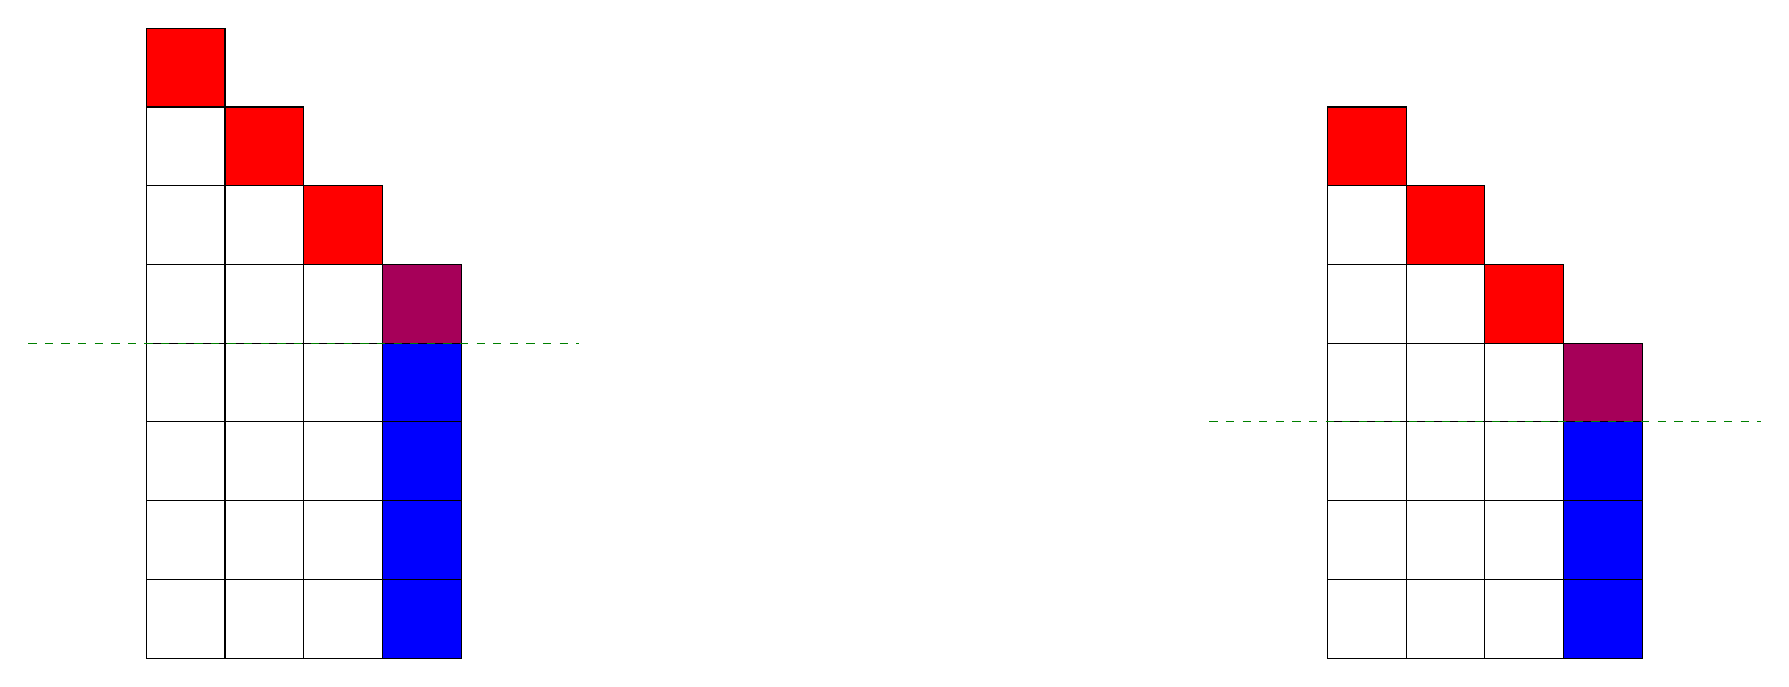
\begin{tikzpicture}
   %% Markierung
   \draw[fill=red] (0,7) rectangle (1,8);
   \draw[fill=red] (1,6) rectangle (2,7);
   \draw[fill=red] (2,5) rectangle (3,6);
   \draw[fill=blue] (3,0) rectangle (4,4);
   \draw[fill=red!65!blue] (3,4) rectangle (4,5);

   %% Diagramm
   \draw[color=black] (0,0) grid (1,8);
   \draw[color=black] (1,0) grid (2,7);
   \draw[color=black] (2,0) grid (3,6);
   \draw[color=black] (3,0) grid (4,5);

   \draw[color=green!50!black,dashed] (-1.5,4) -- (5.5,4);

   %% Markierung
   \draw[fill=red] (15,6) rectangle (16,7);
   \draw[fill=red] (16,5) rectangle (17,6);
   \draw[fill=red] (17,4) rectangle (18,5);
   \draw[fill=blue] (18,0) rectangle (19,3);
   \draw[fill=red!65!blue] (18,3) rectangle (19,4);

   %% Diagramm
   \draw[color=black] (15,0) grid (16,7);
   \draw[color=black] (16,0) grid (17,6);
   \draw[color=black] (17,0) grid (18,5);
   \draw[color=black] (18,0) grid (19,4);

   \draw[color=green!50!black,dashed] (13.5,3) -- (20.5,3);
  \end{tikzpicture}}
 \end{figure}

 Wie wir in den vorhergehenden Fällen bereits gesehen haben, ist es für
 diese Partitionen weder möglich, die Front auf die Schräge zu legen, noch
 die Schräge vor die Front zu stellen. Also haben diese Partitionen keinen
 Partner. Überprüfe das anhand der Beispiele.

 Für welche $n$ gibt es solche Partitionen? Um diese Frage zu beantworten,
 müssen wir die Kästchen zählen. In beiden Fällen haben wir oberhalb
 der gestrichelten Linie $1+2+3+ \dots + (k-1) + k$ Kästchen. Wie du
 vielleicht weißt, kann man diese Summe als
 $$
  \frac{k(k+1)}{2}
 $$ schreiben.\footnote{ Wenn du das noch nicht kennst, informiere dich bei
 Gelegenheit mal über die Gaußsche Summenformel.} Im Fall $\Slope = \Front
 -1$ haben wir unterhalb der gestrichelten Linie $k^2$ viele Kästchen, im
 Fall $\Slope = \Front$ dagegen nur $k(k-1)$ viele Kästchen. Es gibt also
 \mbox{Typ III}-Partitionen genau für die $n$, die sich als
 $$
  n = \frac{k(k+1)}{2} + k^2 = \frac{3k^2+k}{2}
 $$
 oder als
 $$
  n = \frac{k(k+1)}{2} + k(k-1) = \frac{3k^2-k}{2}
 $$
 für ein $k$ schreiben lassen. Das sind exakt die Pentagonalzahlen!
 \end{itemize}

 Fazit: Partner einer Typ I -Partition ist eine Typ II -Partition und
 umgekehrt. Typ III -Partitionen haben keinen Partner. Um
 $p_{dist}^{g-u}(n)=p_{dist}^{g}(n) - p_{dist}^{u}(n)$ zu berechnen, genügt
 es also, (da sich die Säulenanzahl von verpartnerten Typ I und Typ II
 -Partitionen genau um eins unterscheidet) nur die Typ III -Partitionen zu
 kennen. Für die meisten $n$ gibt es keine solche und es gilt
 $p_{dist}^{g-u}(n)=0$. Gibt es doch eine Typ III-Partition von $n$, so ist
 $$
  n = \frac{3k^2 \pm k}{2}
 $$
 für ein $k$, wobei $k$ die Anzahl der Säulen ist und uns somit das
 Vorzeichen liefert, d.\,h. in diesem Fall gilt $p_{dist}^{g-u}(n)=(-1)^k$. Das
 zeigt gerade den eulerschen Pentagonalsatz.
\end{proof}

Puh! Wir haben den eulerschen Pentagonalsatz bewiesen! Aus diesem können wir
direkt folgern, dass
$$
 P(X) \left(1 + \sum_{k=1}^{\infty} (-1)^k \Big(X^{k(3k+1)/2} + X^{k(3k-1)/2}\Big) \right) = 1.
$$
Was bringt uns das? Wir können nun die linke Seite ausmultiplizieren und
anschließend einen Koeffizientenvergleich durchführen. Was ist damit
gemeint? Wir interpretieren beide Seiten der Gleichung als formale Potenzreihe,
so ist z. B.
$$
 1 + \sum_{k=1}^{\infty} (-1)^k \Big(X^{k(3k+1)/2} + X^{k(3k-1)/2} \Big) = 1 - X - X^2 + X^5 + X^7 - X^{12} - X^{15} \pm \dots
$$
Wir werden den $l$-ten Koeffizienten dieser Potenzreihe mit $a_l$ bezeichnen;
wir können dann
$$
  1 + \sum_{k=1}^{\infty} (-1)^k \Big(X^{k(3k+1)/2} + X^{k(3k-1)/2} \Big) = a_0 + a_1 X + a_2 X^2 + \dots = \sum_{l=0}^{\infty} a_l X^l
$$
schreiben. Wir hatten bereits gesehen, dass
$$
a_n =
 \begin{cases}
  (-1)^k, \text{ falls $n$ von  der Form $n = \frac{3k^2 \pm k}{2}$ für ein $k$ und }\\
  \\
  0 \text{ in allen anderen Fällen.}\\
 \end{cases}
$$
Wenn wir nun diese Summe mit $P(X) = p(0) + p(1)X + p(2)X^2 + p(3)X^3 + \dots$
multiplizieren, erhalten wir wieder eine Potenzreihe, nämlich
\footnotesize
$$
 p(0) a_0 + \Big(p(1) a_0 + p(0) a_1  \Big) X + \Big(p(2) a_0 + p(1) a_1 + p(0) a_2  \Big) X^2 + \Big(p(3) a_0 + p(2) a_1 + p(1) a_2 + p(0) a_3 \Big) X^3 + \dots
$$
\normalsize
Der Koeffizient vor $X^t$ in diesem Produkt hat die Form
$$
 \sum_{s=0}^{t} p(t-s) \, a_s,
$$
überlege dir das. Dank des eulerschen Pentagonalsatzes wissen wir aber
gleichzeitig, dass diese Koeffizienten alle verschwinden, bis auf den ersten
vor $X^0$, dieser ist $1$. Wir erhalten also für $t=0$, dass $p(0) \cdot a_0
= 1$ und daraus $p(0) = 1$. Für alle anderen $t > 0$ erhalten wir dagegen,
dass
$$
 \sum_{s=0}^{t} p(t-s) \, a_s = 0.
$$
Diese Gleichungen können wir nun umformen. Unter Ausnutzung von $a_0 = 1$
können wir $p(t)$ auf die andere Seite bringen und erhalten nach langen
Mühen endlich eine Rekursionsformel
\begin{equation}\label{eq_rek}
 p(t) = - \sum_{s=1}^{t} p(t-s) \, a_s.
\end{equation}
für $p(t)$.\\

Mithilfe der folgenden Tabelle sind wir in der Lage, diese Rekursionsformeln
konkret aufzuschreiben.\\

$\begin{array}[h]{c||c|c|c|c|c|c|c|c|c|c|c|c|c|c|c|c}
 k & 1 & 2 & 3 & 4 & 5 & 6 & 7 & 8 & 9 & 10 & 11 & 12 & 13 & 14 & 15 & 16\\
 \hline
 \hline
 \parbox[0pt][3em][c]{0cm}{} \cfrac{3k^2-k}{2} & 1 & 5 & 12 & 22 & 35 & 51 & 70 & 92 & 117 & 145 & 176 & 210 & 247 & 287 & 330 & 376\\
 \hline
 \parbox[0pt][3em][c]{0cm}{} \cfrac{3k^2+k}{2} & 2 & 7 & 15 & 26 & 40 & 57 & 77 & 100 & 126 & 155 & 187 & 222 & 260 & 301 & 345 & 392
\end{array}$\\

\vspace{\baselineskip}

Aus dieser Tabelle können wir nämlich alle Koeffizienten $a_1$, $a_2$, bis
$a_{392}$ der Potenzreihe
$$
 1 + \sum_{k=1}^{\infty} (-1)^k \Big(X^{k(3k+1)/2} + X^{k(3k-1)/2}\Big)  = a_0 + a_1 X + a_2 X^2 + \dots = \sum_{l=0}^{\infty} a_l X^l
$$
ablesen. Wollen wir wissen, welchen Wert $a_m$ für ein $m$ mit $1 \leq m \leq
392$ hat, so über\-prüfen wir als erstes, ob $m$ im rechten unteren Teil
der Tabelle, der durch die doppelten Trennlinien definiert ist, auftaucht. Wenn
nicht, so ist $a_m = 0$. Taucht $m$ dagegen in diesem Teil der Tabelle auf, so
müssen wir überprüfen, in welcher Spalte $m$ steht. Ist die Zahl in der
Spalte von $m$ oberhalb der doppelten Trennlinie gerade, so ist $a_m = 1$, ist
diese Zahl dagegen ungerade, so gilt $a_m = -1$. Wir erhalten (beachte das
Minuszeichen vor der Summe in (\ref{eq_rek}))
$$
 p(n) = p(n-1) + p(n-2) - p(n-5) - p(n-7) + p(n-12) + p(n-15) \pm \dots
$$
Diese Summe scheint in dieser Schreibweise aus unendlich vielen Summanden zu
bestehen, dies ist aber nicht der Fall. Wir wissen nur nicht genau, wie viele
Summanden tatsächlich auftreten. Sobald aber das Argument in $p(\cdot)$
kleiner $0$ ist, bricht diese Summe ab.\\

Mithilfe des Startwerts $p(0) = 1$ können wir nun die ersten Werte der
Partitionsfunktion berechnen:
\begin{align*}
 p(1) &= p(0) &&= 1, \\
 p(2) &= p(1) + p(0) &&= 2, \\
 p(3) &= p(2) + p(1) &&= 3, \\
 p(4) &= p(3) + p(2) &&= 5, \\
 p(5) &= p(4) + p(3) - p(0) &&= 7, \\
 p(6) &= p(5) + p(4) - p(1) &&= 11, \\
 p(7) &= p(6) + p(5) - p(2) - p(0) &&= 15, \\
 p(8) &= p(7) + p(6) - p(3) - p(1) &&= 22, \\
 p(9) &= p(8) + p(7) - p(4) - p(2) &&= 30, \\
 p(10) &= p(9) + p(8) - p(5) - p(3) &&= 42, \\
 p(11) &= p(10) + p(9) - p(6) - p(4) &&= 56, \\
 p(12) &= p(11) + p(10) - p(7) - p(5) + p(0) &&= 77, \\
 \dots\\
 \dots
\end{align*}

Diese Rekursion versetzte Percy Alexander MacMahon noch vor der Entdeckung der
eingangs erwähnten Formel von Hardy, Ramanujan und Rademacher in die Lage,
die ersten $200$ Werte der Partitionsfunktion zu berechnen, was eine
nichttriviale Aufgabe darstellt, denn $p(200) = 3\,972\,999\,029\,388$.

%$p(1000000) = 1471684986358223398631004760609895943484030484439142125334612747351666117418918618276330148873983597555842015374130600288095929387347128232270327849578001932784396072064228659048713020170971840761025676479860846908142829356706929785991290519899445490672219997823452874982974022288229850136767566294781887494687879003824699988197729200632068668735996662273816798266213482417208446631027428001918132198177180646511234542595026728424452592296781193448139994664730105742564359154794989181485285351370551399476719981691459022015599101959601417474075715430750022184895815209339012481734469448319323280150665384042994054179587751761294916248142479998802936507195257074485047571662771763903391442495113823298195263008336489826045837712202455304996382144601028531832004519046591968302787537418118486000612016852593542741980215046267245473237321845833427512524227465399130174076941280847400831542217999286071108336303316298289102444649696805395416791875480010852636774022023128467646919775022348562520747741843343657801534130704761975530375169707999287040285677841619347472368171772154046664303121315630003467104673818$, das sind mehr als $1100$ Stellen.

 \end{document}
